
\section{Desarrollo Enclosure electrónico}
\subsection{Diseño Enclosure electrónico}

En cuanto al diseño de la enclosure para el circuito impreso, este se diseño utilizando el software comercial de diseño asistido por computadora \textbf{Fusion360}. Para el desarrollo final del enclosure se crearon tres modelos durante el proceso de desarrollo. El primero para la versión antigua de la placa de circuito impreso, y los otros dos para el rediseño de la placa. El plano explosionado del modelo de la carcasa y el modelo ensamblado pueden ser vistos en la Figura \ref{fig:carcasa}. También, los archivos de las carcasas desarrolladas se pueden encontrar en los anexos (véase \ref{fig:carcasasVersion}) .
\vspace{5 px}
\begin{figure}[H]
    \centering
    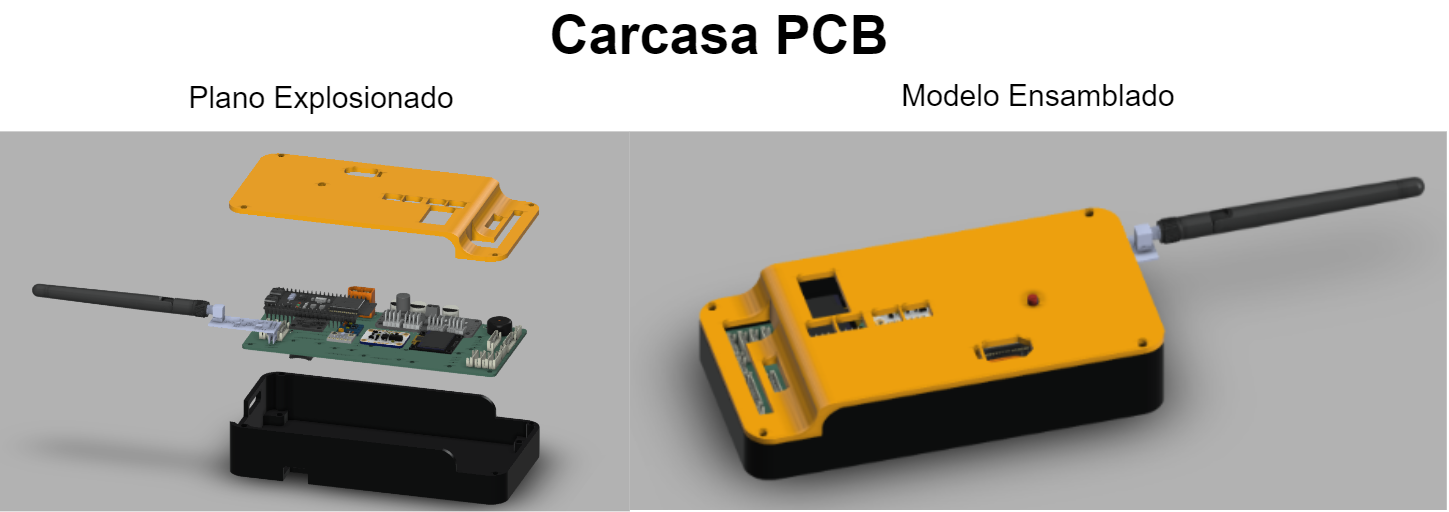
\includegraphics[width=\textwidth]{Imagenes/Metodologia/carcasa.png}
    \caption{Carcasa PCB modelo Final}
    \label{fig:carcasa}
\end{figure}

\\ \\
\subsection{Fabricación Enclosure electrónico}

La fabricación del enclosure electrónico se fabrico utilizando una impresora 3D. Se utilizó PETG para la parte inferior y PLA para la parte superior del chasis. Se utilizó PETG para la parte inferior porque es más resistente que el PLA y puede soportar la tensión mecánica que se asocia con el montaje y la manipulación del usuario, se resalta el uso de insertos metálicos fijados con calor para asegurar correctamente el circuito en la parte inferior de la carcasa. Se utilizó PLA para la parte superior pues esta no requiere de gran resistencia mecánica asociada a su uso y tiene menor densidad. El montaje y producto final se puede observar en \ref{fig:ensamble}. 


\begin{figure}[H]
    \centering
    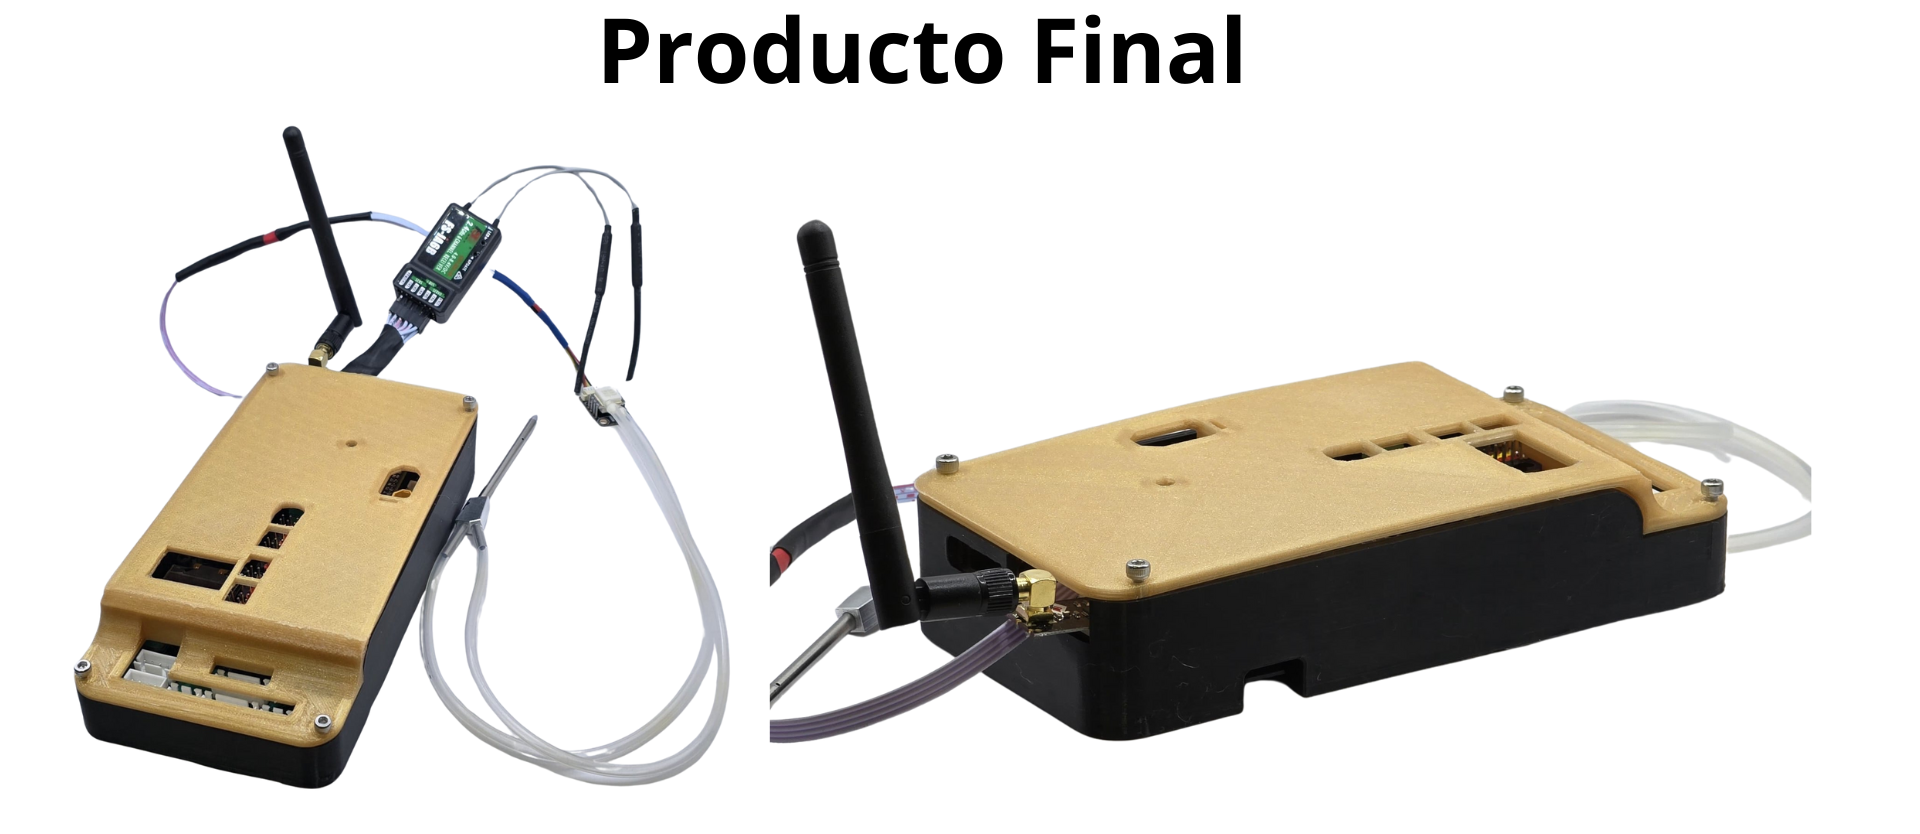
\includegraphics[width=12 cm]{Imagenes/Metodologia/producto final.png}
    \caption{Producto Final ensamblado}
    \label{fig:ensamble}
\end{figure}


